\section{Testing}

The project was tested using the \textbf{Jest} framework, a testing tool that enabled us to test the backend.
Our testing approach was based on the \textbf{DD} as much as possible, given the time constraints.
\hfill \\ \hfill \\
First, we tested the most critical component, the \textbf{Query Manager}, through indirect testing,
with a coverage rate of nearly 100\%. Other components,
which mostly serve as wrappers for the Query Manager, were tested using modular tests provided by Jest.
\hfill \\ \hfill \\
To ensure that our tests didn't affect the data in the database,
we created a Query Manager method that executes a callback function and,
regardless of its outcome, rolls back changes using a \textbf{ROLLBACK SQL} operation.

\subsection{Relevant Test Cases}

The following relevant test cases were implemented:
\begin{itemize}
    \item User creation for CPO and Drivers, including sign-up, code verification, and login
    \item EVCP creation and deletion by the CPO, along with the creation of new CP and related sockets
    \item Driver reservation creation
    \item Driver search for EVCP
    \item CPO creation of rates and special offers
    \item CPO selection of a DSO, including searching for available DSOs and choosing one
\end{itemize}
\subsection{Outcomes}

A summary of the testing outcomes can be found in the Testing Report generated by Jest and located in the /coverage folder of the project. Detailed information is available in the report.

\begin{figure}[H]
    \centering
    \vspace{0.5cm}
    \hspace*{-1.5cm}
    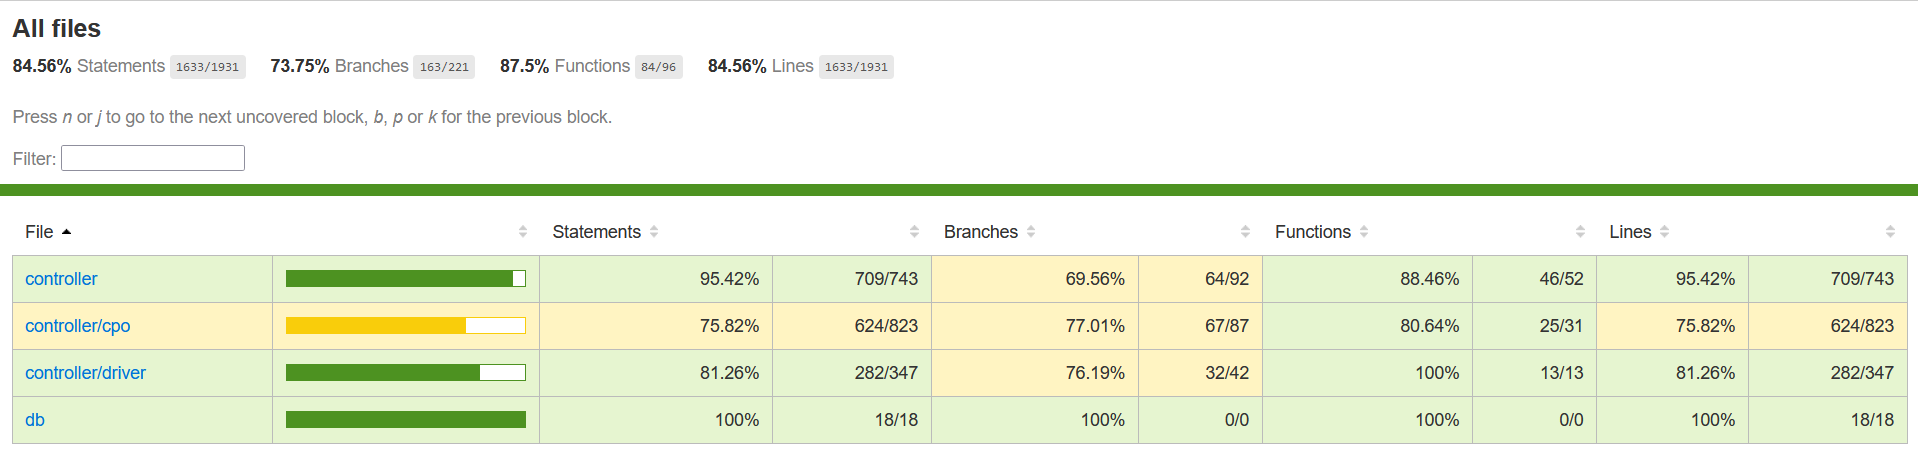
\includegraphics[width = 1.2\textwidth]{src/coverage_report.png}
    \caption{Summary Coverage Report}
\end{figure}